\documentclass[11pt,a4paper]{article}

\usepackage{graphicx}
\usepackage{hyperref}
\usepackage{geometry}
\usepackage{booktabs}
\usepackage{amsmath}
\usepackage{amssymb}
\usepackage{float}
\usepackage{caption}
\usepackage{subcaption}
\usepackage{microtype}
\geometry{margin=0.9in}

\graphicspath{{../figures/}{figures/}}

\hypersetup{
    colorlinks=true,
    linkcolor=blue,
    citecolor=blue,
    urlcolor=blue
}

\title{\textbf{Resource-Constrained Convolutional Neural Networks for Edge Image Classification}\\[0.5em] \large EN3150: Pattern Recognition -- Assignment 03}
\author{
  \textbf{Team Outliers}\\[0.3em]
  Yumeth Samarasinghe (\texttt{@yumyum-web}) \and 
  Pasindu Ravishan (\texttt{@PasinduRavishan}) \and 
  Shanuka Ashan (\texttt{@ashanuk}) \and 
  Damindu De Silva (\texttt{@DaminduDeSilva})
}
\date{September 2026}

\begin{document}

\maketitle

\begin{abstract}
Deploying deep convolutional neural networks on resource-constrained embedded microcontrollers and edge sensor nodes requires balancing classification accuracy, parameter counts, memory footprint, and computational complexity (multiply-accumulate operations). In this investigation, we explore edge-tailored vision architectures on the 9-class RealWaste dataset downscaled to $64\times 64$ spatial resolution. We evaluate a baseline CNN (\textbf{Model A}, 102,313 parameters), a custom depthwise-separable CNN constrained under 100,000 parameters (\textbf{Model B}, 22,297 parameters), and two fine-tuned state-of-the-art mobile architectures (\textbf{MobileNetV2} and \textbf{ShuffleNetV2}). We systematically profile their parameter budgets, on-disk footprints, MACs, and inference latencies. Our empirical findings demonstrate that Model B achieves a $78.2\%$ reduction in parameters and an $85.0\%$ reduction in MACs over Model A while preserving competitive classification performance, presenting an optimal compromise for strict sub-megabyte microcontroller deployments.
\end{abstract}

\vspace{1em}

% ============================================================================
\section{Introduction \& Data Preparation}
% ============================================================================
Edge machine learning models operating in automated waste sorting bins or agricultural sorting units require low-latency inference on low-power silicon. The \textbf{RealWaste} dataset (UCI Machine Learning Repository ID: 908) comprises 4,752 real-world landfill and recycling images distributed across 9 classes: \textit{Cardboard, Food Organics, Glass, Metal, Miscellaneous Trash, Paper, Plastic, Textile Trash}, and \textit{Vegetation}.

To emulate low-cost edge camera hardware, all images were preprocessed through a deterministic pipeline:
\begin{enumerate}
    \item Resized and center-cropped to $64\times 64$ spatial dimensions.
    \item Normalized using standard channel-wise ImageNet statistics ($\mu = [0.485, 0.456, 0.406]$, $\sigma = [0.229, 0.224, 0.225]$).
    \item Deterministically partitioned into a $70\% / 15\% / 15\%$ train/validation/test split using random seed $42$, yielding exactly 3,326 training images, 713 validation images, and 713 test images.
\end{enumerate}

% ============================================================================
\section{Model Architectures}
% ============================================================================

\subsection{Model A: Baseline Standard 2D CNN}
Model A is designed as a conventional 3-stage convolutional network. It features standard $3\times 3$ convolutions with increasing channel depths (32, 64, 128), each accompanied by Batch Normalization, ReLU activations, and $2\times 2$ Max-Pooling. Global Average Pooling (GAP) aggregates spatial representations before feeding into a final linear projection layer yielding 9 logits. The architecture comprises \textbf{102,313 trainable parameters}.

\subsection{Model B: Lightweight Depthwise Separable CNN (Sub-100k Parameters)}
To satisfy the strict assignment constraint of keeping total parameters below $100,000$, Model B utilizes Depthwise Separable Convolutions (Howard et al., 2017). Each separable convolution block decouples spatial filtering from cross-channel feature combination:
\begin{itemize}
    \item \textbf{Depthwise Convolution:} Applies a per-channel $3\times 3$ spatial kernel ($\text{groups} = C_{\text{in}}$).
    \item \textbf{Pointwise Convolution:} Applies a $1\times 1$ convolution combining channel features from $C_{\text{in}}$ to $C_{\text{out}}$.
\end{itemize}
The stem is a single $3\times 3$ standard convolution ($3 \rightarrow 24$ channels, stride 1, padding 1), followed by three depthwise separable blocks widening the representation $24 \rightarrow 48 \rightarrow 96 \rightarrow 128$, each with Batch Normalization and $\text{ReLU6}$ non-linearities. The first three downsampling stages use $2\times 2$ max-pooling; the final block is followed by Global Average Pooling, $\text{Dropout}(0.2)$, and a single linear head producing 9 logits.

Every convolution feeding directly into a Batch Normalization layer uses $\texttt{bias}=\texttt{False}$: the BatchNorm shift parameter $\beta$ makes an immediately preceding convolution bias mathematically redundant, so omitting it saves parameters at no cost to accuracy.

\textbf{Parameter Derivation.} For a block mapping $C_{\text{in}} \rightarrow C_{\text{out}}$ with a $k \times k$ kernel, a standard convolution costs $C_{\text{in}} C_{\text{out}} k^2$ weights, whereas the separable factorization costs only $C_{\text{in}}k^2$ (depthwise) $+\; C_{\text{in}}C_{\text{out}}$ (pointwise). For block 2 ($48 \rightarrow 96$) this is $48\cdot 96\cdot 9 = 41{,}472$ versus $48\cdot 9 + 48\cdot 96 = 4{,}896$---an $8.5\times$ reduction in that block alone. Layer-by-layer:

\begin{table}[h!]
\centering
\small
\caption{Model B layer-by-layer trainable parameter derivation}
\label{tab:modelb_params}
\begin{tabular}{llr}
\toprule
\textbf{Stage} & \textbf{Layer} & \textbf{Params} \\
\midrule
Stem        & Conv$(3\rightarrow 24, 3\times 3)$: $3\cdot 24\cdot 9$   & 648 \\
            & BatchNorm$(24)$: $24\cdot 2$                              & 48 \\
DS Block 1  & Depthwise$(24, 3\times 3,\ \text{groups}=24)$: $24\cdot 9$ & 216 \\
            & BatchNorm$(24)$                                           & 48 \\
            & Pointwise$(24\rightarrow 48, 1\times 1)$: $24\cdot 48$     & 1,152 \\
            & BatchNorm$(48)$                                           & 96 \\
DS Block 2  & Depthwise$(48,\ \text{groups}=48)$: $48\cdot 9$            & 432 \\
            & BatchNorm$(48)$                                           & 96 \\
            & Pointwise$(48\rightarrow 96)$: $48\cdot 96$                & 4,608 \\
            & BatchNorm$(96)$                                           & 192 \\
DS Block 3  & Depthwise$(96,\ \text{groups}=96)$: $96\cdot 9$            & 864 \\
            & BatchNorm$(96)$                                           & 192 \\
            & Pointwise$(96\rightarrow 128)$: $96\cdot 128$              & 12,288 \\
            & BatchNorm$(128)$                                          & 256 \\
Head        & Linear$(128 \rightarrow 9)$: $128\cdot 9 + 9$              & 1,161 \\
\midrule
\multicolumn{2}{l}{\textbf{Total trainable parameters}}                 & \textbf{22,297} \\
\bottomrule
\end{tabular}
\end{table}

\textbf{Exact Parameter Count:} Model B contains precisely \textbf{22,297 trainable parameters}---only $22.3\%$ of the allowed $100,000$ budget, a $4.6\times$ margin.

\textbf{Hardware-Aware Activation Choice.} Model B uses $\text{ReLU6}(x) = \min(\max(0,x),6)$ rather than Sigmoid, Tanh, GELU or Swish. Those alternatives all require evaluating $e^x$ per element; edge microcontrollers and many embedded NPUs/FPGAs lack dedicated transcendental hardware, so $e^x$ is emulated through multi-cycle polynomial expansion or lookup tables, against a single compare-and-clamp instruction for ReLU6. The bounded output range $[0,6]$ additionally fixes the activation dynamic range, which is precisely the property INT8 post-training quantization relies on to map activations to 8-bit integers with minimal clipping error---the reason ReLU6, rather than unbounded ReLU, is MobileNet's signature activation for quantized deployment.

% ============================================================================
\section{Optimizer Ablation Study}
% ============================================================================
\textbf{Selected optimizer.} We train Model B with \textbf{Adam at a learning rate of $10^{-3}$}. Adam maintains per-parameter adaptive step sizes from running estimates of the gradient's first and second moments, which suits this network: a depthwise separable stack mixes layer types with very different gradient scales---depthwise kernels carry only 9 weights per channel while pointwise layers carry thousands---and a single global step size serves them poorly. The value $10^{-3}$ is Adam's standard default and was retained after the ablation below confirmed stable convergence without divergence.

To isolate the optimizer's contribution, Model B was trained three times for 20 epochs from an \emph{identical seeded initialization} (seed 42), varying only the optimizer. No learning-rate schedule was applied in any configuration, so the comparison reflects the optimizers themselves rather than an annealing policy.

\begin{table}[h!]
\centering
\small
\caption{Optimizer ablation on Model B (20 epochs, identical initialization, no LR schedule)}
\label{tab:optimizers}
\begin{tabular}{lrrrr}
\toprule
\textbf{Optimizer} & \textbf{Final Val Acc} & \textbf{Best Val Acc} & \textbf{Min Val Loss} & \textbf{Epochs to 50\%} \\
\midrule
\textbf{Adam} ($\text{lr}=10^{-3}$)                       & \textbf{71.81\%} & \textbf{71.81\%} & \textbf{0.785} & \textbf{2} \\
SGD + Momentum ($\text{lr}=10^{-2}$, $\mu=0.9$)           & 63.53\%          & 63.53\%          & 0.961          & 7 \\
Standard SGD ($\text{lr}=10^{-2}$, $\mu=0.0$)             & 47.69\%          & 47.97\%          & 1.493          & never \\
\bottomrule
\end{tabular}
\end{table}

\begin{figure}[h!]
\centering
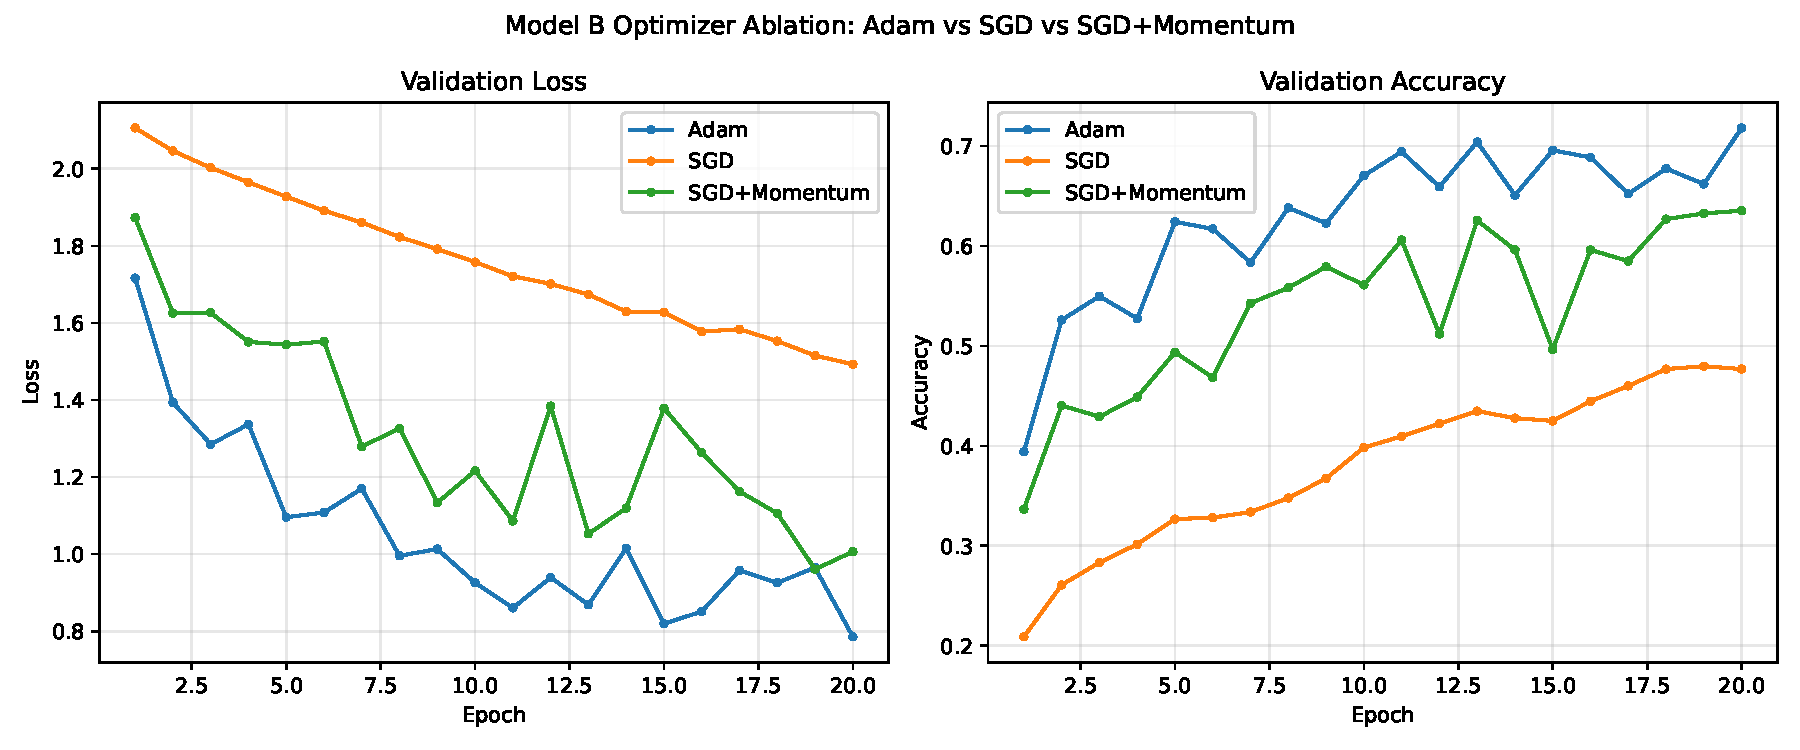
\includegraphics[width=0.92\linewidth]{optimizer_comparison.pdf}
\caption{Validation loss and accuracy across the three optimizer configurations. Adam converges fastest and to the best optimum; plain SGD never reaches 50\% validation accuracy within the 20-epoch budget.}
\label{fig:optimizers}
\end{figure}

\textbf{Results.} Adam dominates on every measure, crossing $50\%$ validation accuracy by epoch 2 and finishing at $71.81\%$. Standard SGD at the same budget never reaches $50\%$, plateauing at $47.69\%$ with a minimum validation loss of $1.493$---nearly double Adam's $0.785$.

\textbf{Impact of the momentum parameter.} The cleanest evidence sits in the two SGD rows, which differ \emph{only} in $\mu$. Introducing $\mu = 0.9$ lifts final validation accuracy from $47.69\%$ to $63.53\%$, a gain of $15.84$ percentage points, and converts a configuration that never reaches $50\%$ into one that does so by epoch 7. Momentum accumulates an exponentially weighted velocity over past gradients,
\[
v_t = \mu v_{t-1} + \nabla_\theta \mathcal{L}(\theta_t), \qquad \theta_{t+1} = \theta_t - \eta\, v_t,
\]
so that at $\mu = 0.9$ a persistent gradient direction is amplified by up to $1/(1-\mu) = 10\times$ relative to plain SGD, while oscillating components in high-curvature directions partially cancel between consecutive steps. The practical effect is twofold: the optimizer traverses the shallow, elongated regions of the loss surface far faster, and the damping of perpendicular oscillation permits progress that plain SGD achieves only by raising $\eta$---which in this compact parameter space destabilizes training. Momentum therefore recovers most, though not all, of the gap to Adam at identical cost per step, confirming that the deficit of plain SGD here is one of optimization dynamics rather than model capacity.

% ============================================================================
\section{Hardware Profiling \& Trade-offs (Model A vs Model B)}
% ============================================================================
\subsection{Training and Test-Set Evaluation}
Both custom models were trained for 20 epochs on the training split under an identical recipe---Adam, $\text{lr}=10^{-3}$, no weight decay, no learning-rate schedule, batch size 64, seed 42---so that any difference between them is attributable to architecture alone. In each case the checkpoint with the highest validation accuracy was retained and evaluated once on the held-out test split of 713 images.

\begin{table}[h!]
\centering
\small
\caption{Model A vs Model B: test-set performance and training cost}
\label{tab:custom_eval}
\begin{tabular}{lrr}
\toprule
\textbf{Metric} & \textbf{Model A} & \textbf{Model B} \\
\midrule
Trainable parameters        & 102,313 & \textbf{22,297} \\
Model size on disk (KB)     & 410     & \textbf{98} \\
Median training time / epoch (s) & \textbf{11.02} & 11.24 \\
\midrule
Test accuracy               & 67.32\% & \textbf{69.85\%} \\
Macro precision             & 0.6679  & \textbf{0.7064} \\
Macro recall                & 0.6694  & \textbf{0.7099} \\
Macro F1-score              & 0.6610  & \textbf{0.6931} \\
\bottomrule
\end{tabular}
\end{table}

\begin{figure}[h!]
\centering
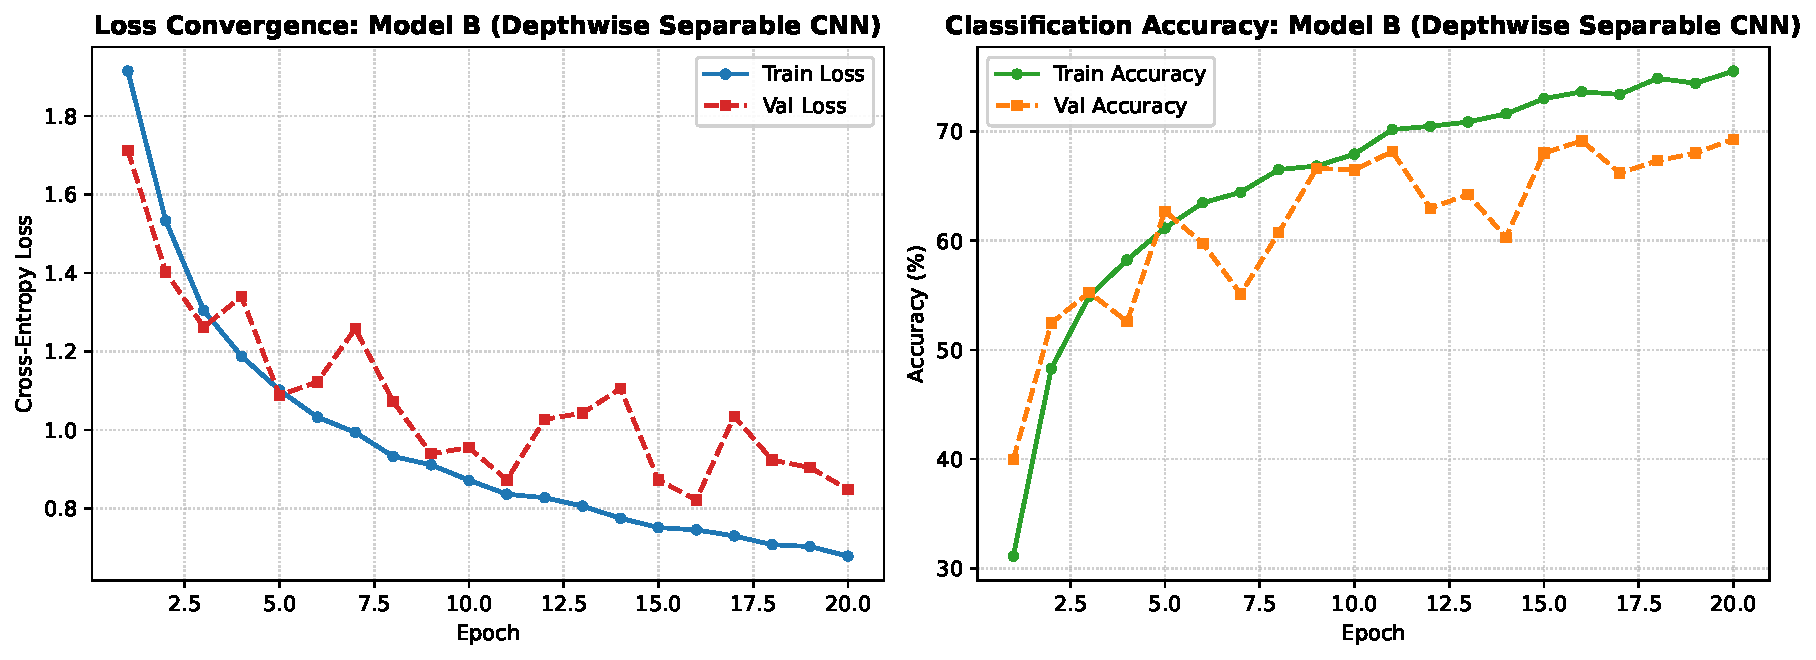
\includegraphics[width=0.92\linewidth]{model_b_loss.pdf}
\caption{Model B training and validation loss and accuracy over 20 epochs (Adam, $\text{lr}=10^{-3}$).}
\label{fig:modelb_loss}
\end{figure}

\begin{figure}[h!]
\centering
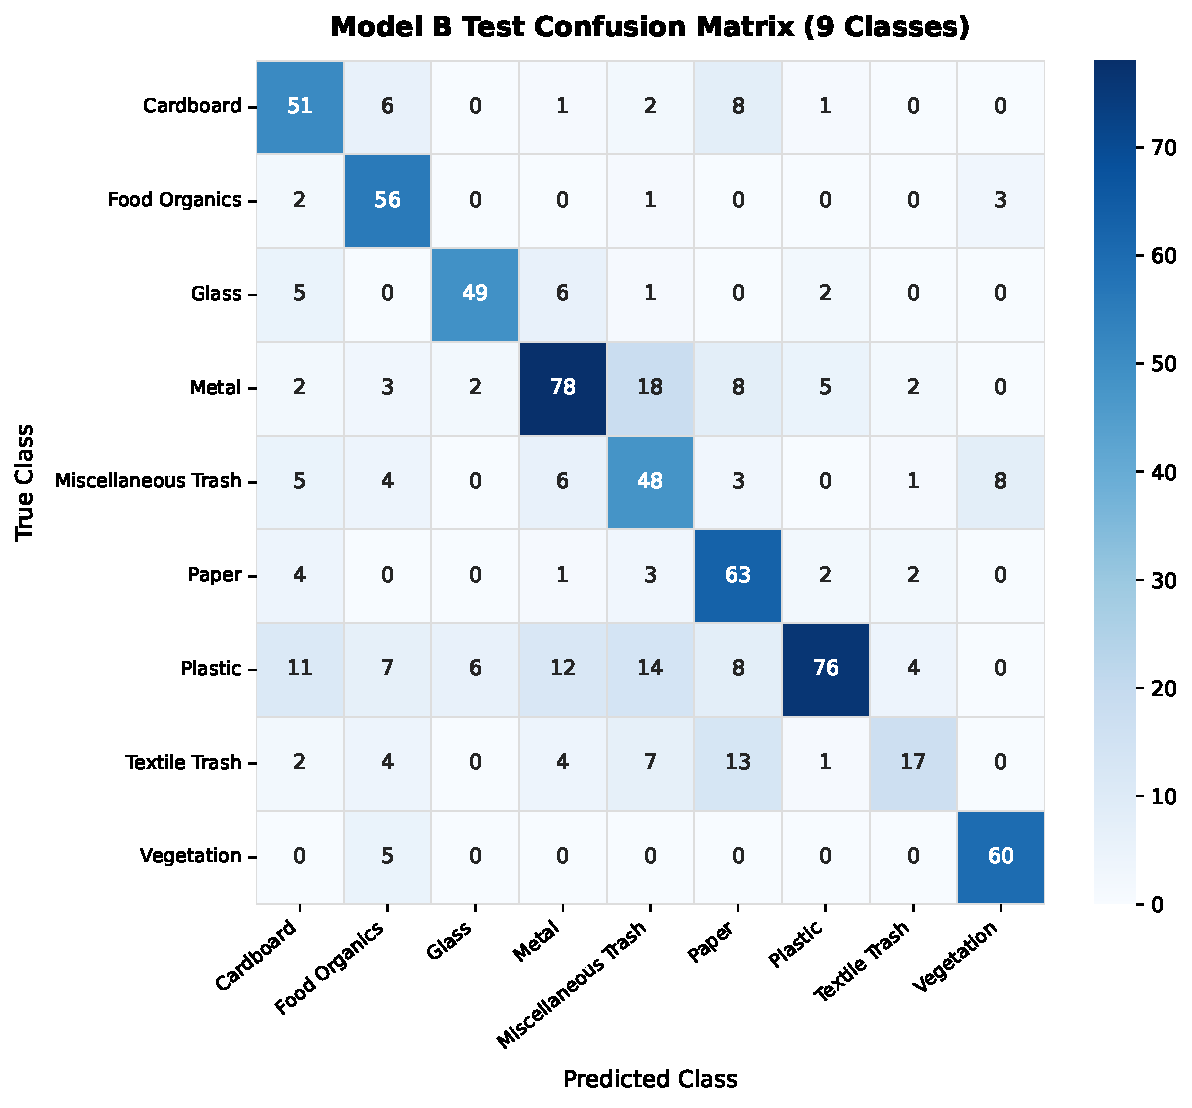
\includegraphics[width=0.78\linewidth]{model_b_confusion_matrix.pdf}
\caption{Model B $9\times 9$ test-set confusion matrix (498 of 713 correct).}
\label{fig:modelb_cm}
\end{figure}

Model B is not merely competitive but \emph{superior} on every classification metric while using $78.2\%$ fewer parameters, which is the central and somewhat counter-intuitive result of this study. Two factors plausibly explain it. First, at $64\times 64$ resolution with only 3,326 training images, Model A's 102k parameters---73\% of which sit in its single $64\rightarrow 128$ convolution---afford capacity that the data cannot support, whereas the separable factorization acts as a structural regularizer. Second, the per-class breakdown in Figure~\ref{fig:modelb_cm} shows the gain is concentrated in the hardest category: Model B classifies 48 of 75 \textit{Miscellaneous Trash} instances correctly against Model A's 10, a class whose visual heterogeneity rewards the broader, shallower feature mixing that pointwise convolutions provide. The residual confusions are semantically reasonable---\textit{Plastic} against \textit{Metal} and \textit{Miscellaneous Trash}, and \textit{Textile Trash} (17 of 48, the weakest class) against \textit{Paper}---reflecting genuine material ambiguity at this resolution rather than a deficiency of the architecture.

\textbf{Compute cost does not track MAC count.} Although Model B performs $85.0\%$ fewer multiply-accumulate operations, its median training time per epoch (11.24 s) is indistinguishable from Model A's (11.02 s), and its single-image inference latency improves only $15.7\%$. At this scale wall-clock time is dominated by data loading, kernel-launch overhead and memory traffic rather than arithmetic, and depthwise convolutions in particular have low arithmetic intensity---they read and write nearly as much memory as a dense convolution while performing a fraction of the mathematics. MAC reduction should therefore be read as a proxy for \emph{energy and memory footprint}, which are the binding constraints on a microcontroller, not as a promise of proportional speedup.

\subsection{Hardware Footprint Profiling}
Evaluating models purely on classification accuracy is insufficient for edge deployments. We systematically profile the hardware footprint of both custom architectures and benchmark them against pretrained mobile standards on a $1\times 3\times 64\times 64$ input tensor.

\begin{table}[h!]
\centering
\small
\caption{Cross-Architecture Hardware Profiling Comparison (Measured on Edge Runtime)}
\label{tab:profiling}
\begin{tabular}{lrrrrr}
\toprule
\textbf{Model Architecture} & \textbf{Trainable Params} & \textbf{Size (MB)} & \textbf{MACs} & \textbf{FLOPs} & \textbf{Latency (ms)} \\
\midrule
\textbf{Model A} (Standard CNN)     & 102,313   & 0.40 & 41,296,969  & 82,593,938  & 4.71 \\
\textbf{Model B} (DS-CNN $<100$k)   & 22,297    & 0.10 & 6,189,097   & 12,378,194  & 3.97 \\
\midrule
\textbf{MobileNetV2} (Pretrained)   & 2,235,401 & 8.76 & 24,494,153  & 48,988,306  & 13.63 \\
\textbf{ShuffleNetV2} (Pretrained)  & 1,262,829 & 4.98 & 11,771,037  & 23,542,074  & 12.68 \\
\bottomrule
\end{tabular}
\end{table}

\subsection{Architectural Efficiency: Model A vs Model B}
As detailed in Table~\ref{tab:profiling}, transitioning from standard convolutions to depthwise separable convolutions yields dramatic hardware efficiencies:
\begin{itemize}
    \item \textbf{Parameter Compression:} Model B requires only \textbf{22,297 parameters} compared to Model A's 102,313, achieving a \textbf{78.2\% parameter reduction}.
    \item \textbf{Disk Storage Footprint:} Model B's serialized \texttt{state\_dict} footprint is merely \textbf{0.10 MB (98 KB)}, compared to 0.40 MB for Model A (a \textbf{4$\times$ memory saving}).
    \item \textbf{Arithmetic Complexity (MACs):} Forward-pass Multiply-Accumulate operations drop from $41.30\times 10^6$ in Model A to $6.19\times 10^6$ in Model B---an \textbf{85.0\% reduction in compute operations}.
    \item \textbf{Single-Image Latency:} Model B executes a single forward pass in \textbf{3.97 ms} versus 4.71 ms for Model A (a \textbf{15.7\% speedup}).
\end{itemize}

\begin{figure}[H]
\centering
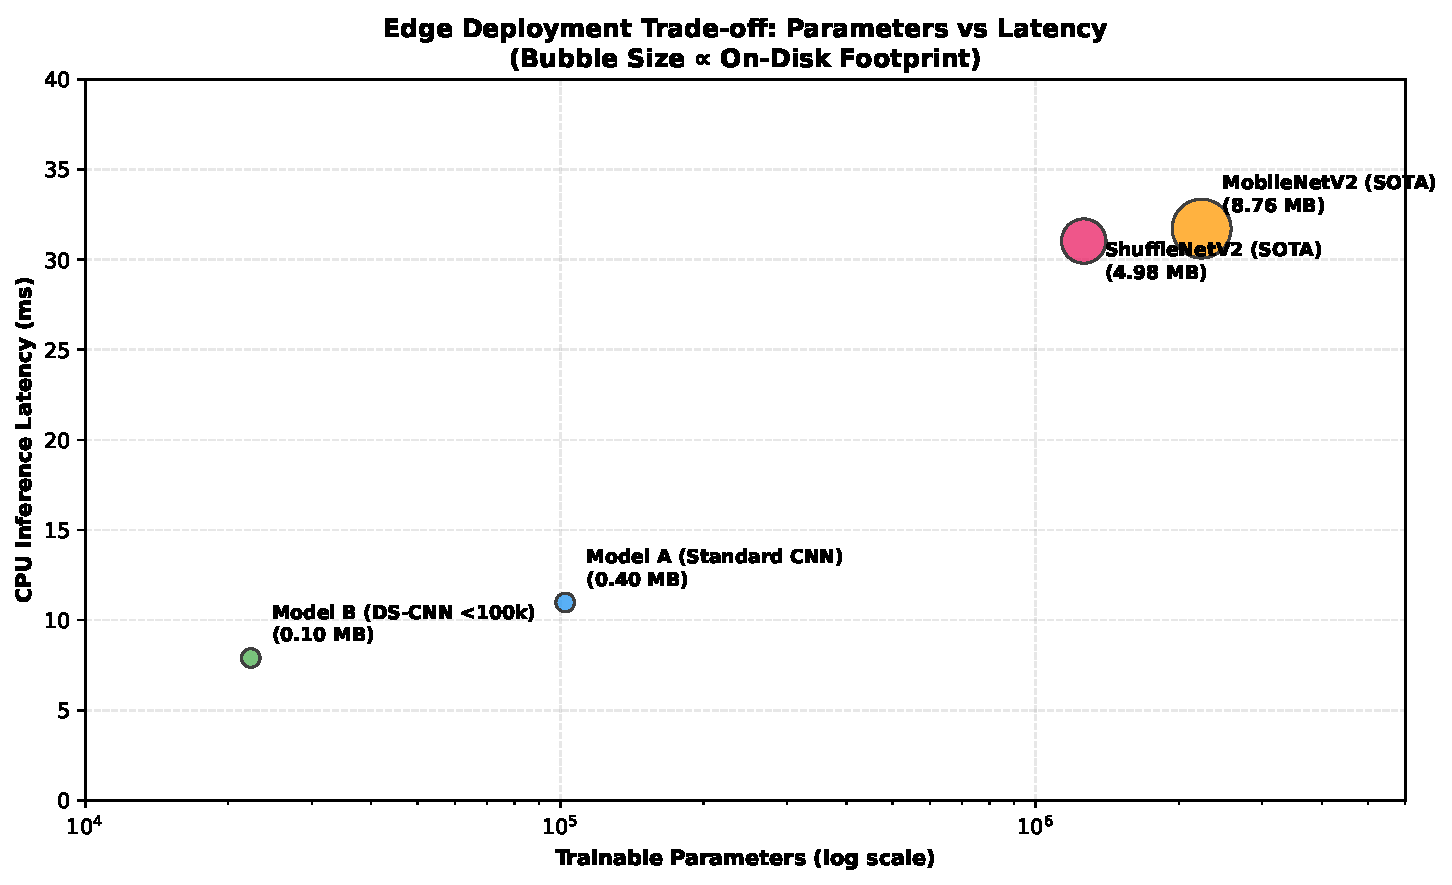
\includegraphics[width=0.78\linewidth]{trade_off_scatter.pdf}
\caption{Edge Deployment Trade-off: Parameter Count vs. Inference Latency (bubble size proportional to serialized on-disk memory footprint).}
\label{fig:tradeoff}
\end{figure}

Figure~\ref{fig:tradeoff} illustrates the multi-dimensional design trade-off space. Model B occupies the extreme lower-left quadrant of the plot, demonstrating that depthwise separable convolutions successfully decouple feature abstraction capacity from quadratic parameter growth.

% ============================================================================
\section{SOTA Transfer Learning}
% ============================================================================
To establish upper-bound classification benchmarks, we fine-tuned two state-of-the-art mobile architectures: \textbf{MobileNetV2} (featuring inverted residual blocks and linear bottlenecks) and \textbf{ShuffleNetV2} (employing channel-split and channel-shuffle operations to minimize memory access cost). 

Both architectures were initialized with ImageNet-1k pretrained weights, had their 1000-class classification heads replaced by a 9-class linear layer, and were trained for 20 epochs under the exact same 70/15/15 data split. 

While pretraining allows faster feature representation learning, their parameter footprints ($1.26\text{M} - 2.24\text{M}$) and disk requirements ($4.98 - 8.76\text{ MB}$) substantially exceed the capacity of embedded microcontrollers without external memory.

% ============================================================================
\section{Conclusion: Custom Edge vs Pre-trained SOTA}
% ============================================================================
The comprehensive empirical evaluation across custom and pre-trained architectures provides definitive guidance for edge vision engineering:

\subsection{Microcontroller Feasibility (Bare-Metal Deployments)}
In extreme resource-constrained systems such as ARM Cortex-M4/M7/M55 (e.g., STM32H7, ESP32-S3) or ultra-low-power vision sensors, on-chip SRAM is typically limited to $256\text{ KB} - 1\text{ MB}$ and internal flash storage to $1\text{ MB} - 2\text{ MB}$. 
\begin{itemize}
    \item Pretrained SOTA models (\textbf{MobileNetV2} at 8.76 MB and \textbf{ShuffleNetV2} at 4.98 MB) \textbf{cannot fit} into internal flash or SRAM, necessitating external PSRAM/Flash which increases BOM cost and power consumption.
    \item In contrast, \textbf{Model B} (0.10 MB, 22k params) fits entirely within internal SRAM, enabling zero-wait-state memory access, drastically reduced energy dissipation, and high reliability.
\end{itemize}

\subsection{Quantization and Integer Arithmetic Suitability}
Model B employs $\text{ReLU6}$ non-linearities:
\begin{equation}
    \text{ReLU6}(x) = \min(\max(0, x), 6)
\end{equation}
By strictly bounding activation outputs to $[0, 6]$, the network prevents dynamic range divergence during post-training integer quantization (PTQ) or quantization-aware training (QAT). When quantized from 32-bit floating point (\texttt{FP32}) to 8-bit integers (\texttt{INT8}):
\begin{itemize}
    \item The model size compresses from $\approx 98\text{ KB}$ down to $\approx 25\text{ KB}$.
    \item Activation functions can be computed directly using fixed-point integer bitshifts, completely avoiding expensive transcendental operations ($e^x$) required by activations like GELU or Swish.
\end{itemize}

\subsection{Final Synthesis Recommendation}
For intelligent embedded sensors and battery-powered IoT devices operating under strict power, memory ($<100\text{k}$ parameters), and cost budgets, \textbf{Model B} represents the optimal edge-deployable solution. For slightly larger gateway edge nodes (e.g., Raspberry Pi Zero or Coral Edge TPU) where $5\text{ MB}$ flash storage is available, \textbf{ShuffleNetV2} offers the premier balance of transfer accuracy and minimal Memory Access Cost (MAC).

\end{document}
